
%\RequirePackage{pdf15}

\documentclass{beamer}

\usepackage[utf8]{inputenc}

\usepackage{mystyle}

\usepackage{tikz}
\usepackage{pgfplots}
\usepackage{subcaption}

\usepackage{natbib}
\bibliographystyle{apalike}
%\usepackage[style=authortitle,backend=biber]{biblatex}
%\addbibresource{anthology.bib}
%\addbibresource{emnlp2020.bib}
\renewcommand{\footnotesize}{\scriptsize}

\newcommand{\bigCI}{\mathrel{\text{\scalebox{1.07}{$\perp\mkern-10mu\perp$}}}}

\usepackage{tikz-dependency}
\usetikzlibrary{shapes.arrows, positioning, fit, bayesnet,
    arrows,backgrounds,patterns,matrix,calc,shadows,plotmarks,
    shapes,positioning,automata,positioning,spy,scopes,chains,decorations,decorations.pathreplacing}

\newcommand{\FancyUpArrow}{
\begin{tikzpicture}[baseline=-0.3em]
\node[single arrow,draw,rotate=90,single arrow head extend=0.2em,inner
ysep=0.2em,transform shape,line width=0.05em,top color=green,bottom color=green!50!black] (X){};
\end{tikzpicture}}
\newcommand{\FancyDownArrow}{
\begin{tikzpicture}[baseline=-0.3em]
\node[single arrow,draw,rotate=-90,single arrow head extend=0.2em,inner
ysep=0.2em,transform shape,line width=0.05em,top color=red,bottom color=red!50!black] (X){};
\end{tikzpicture}}

\AtBeginSection[]{
  \begin{frame}
  \vfill
  \centering
  \begin{beamercolorbox}[sep=8pt,center,shadow=true,rounded=true]{title}
    \usebeamerfont{title}\insertsectionhead\par%
  \end{beamercolorbox}
  \vfill
  \end{frame}
}

% quotes
\usepackage[style=british]{csquotes}

\def\signed #1{{\leavevmode\unskip\nobreak\hfil\penalty50\hskip1em
  \hbox{}\nobreak\hfill #1%
  \parfillskip=0pt \finalhyphendemerits=0 \endgraf}}

\newsavebox\mybox
\newenvironment{aquote}[1]
  {\savebox\mybox{#1}\begin{quote}\openautoquote\hspace*{-.7ex}}
  {\unskip\closeautoquote\vspace*{1mm}\signed{\usebox\mybox}\end{quote}}

%Information to be included in the title page:
\title{Word Games}
\author{J Chiu}

\setbeamertemplate{navigation symbols}{} 
\setbeamertemplate{footline}[frame number]

\begin{document}

\begin{frame}[plain]
\titlepage
\end{frame}

\begin{frame}
\frametitle{Dialogue}
\begin{itemize}
\item Communication is rarely unambiguous
    \begin{itemize}
    \item Ambiguity resolution through dialogue
    \item Clarification questions
    \end{itemize}
\item Interactive, symmetric reference games
    \begin{itemize}
    \item Isolates ambiguity resolution
    \item Both give and request information
    \end{itemize}
\end{itemize}
\end{frame}

\begin{frame}
\frametitle{Games}

\begin{columns}
\begin{column}{0.5\textwidth}
\centering
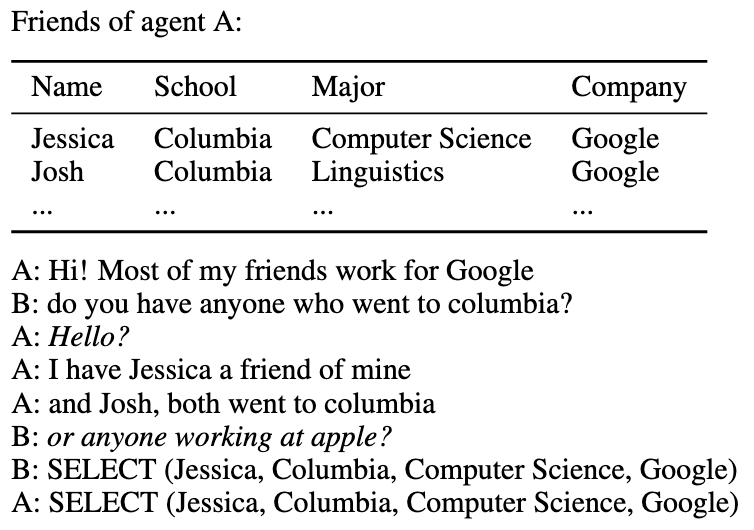
\includegraphics[width=2in]{img/mf.png}
\end{column}
\begin{column}{0.5\textwidth}
\centering
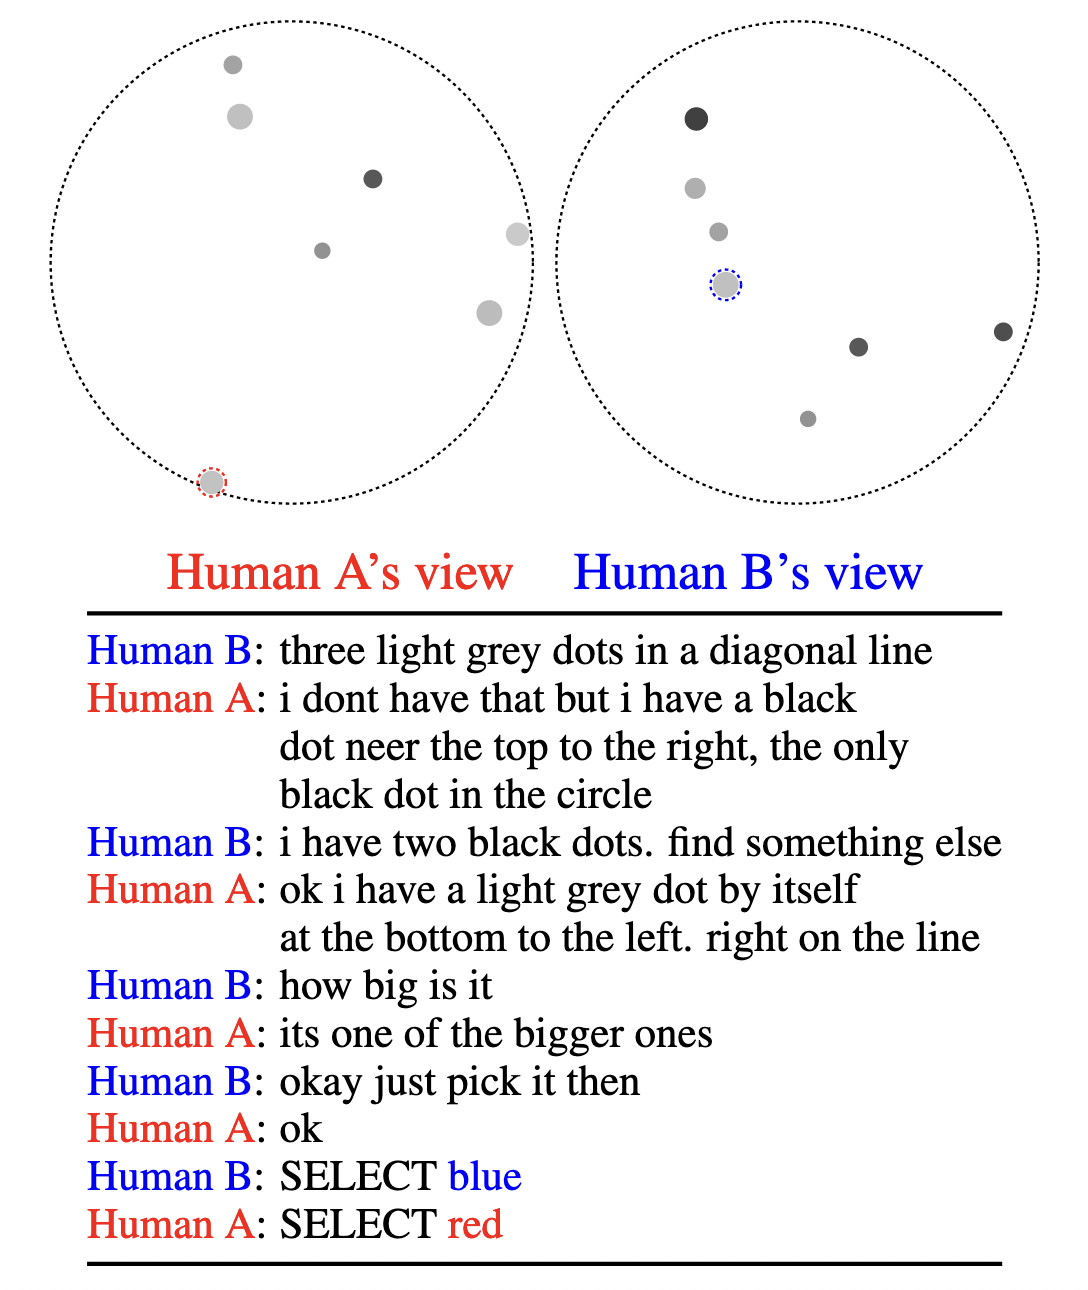
\includegraphics[width=2in]{img/oc.png}
\end{column}
\end{columns}

\vspace{2em}
\centering
Mutual Friends and OneCommon
\end{frame}

\begin{frame}
\frametitle{Issue: Poor neural reasoning}
From Mutual Friends: Neural + Human
\begin{itemize}
\item A: Know anyone who likes chess?
\item B: None of my friends like chess.
\item (conversation continues)
\item A: Crocheting?
\item B: None like crocheting.
\item A: Chess?
\item B: None like chess either, haha.
\end{itemize}
\end{frame}

\begin{frame}
\frametitle{Issue: Poor neural reasoning}
\centering
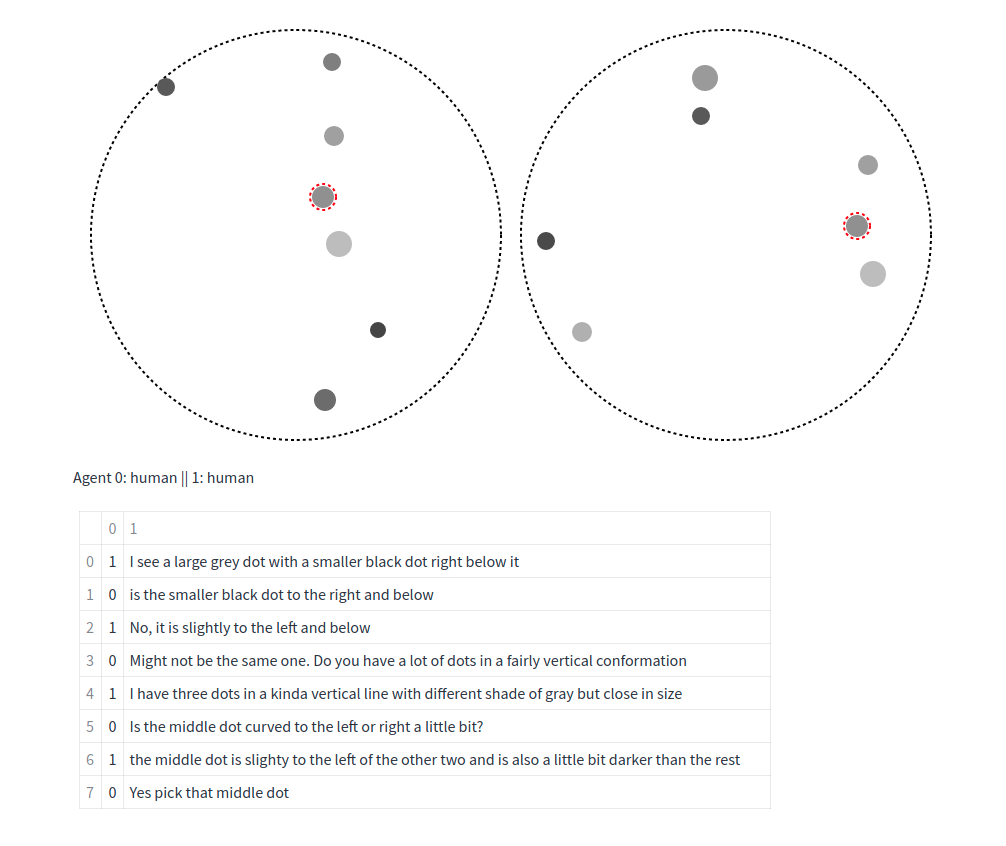
\includegraphics[height=3in]{img/oc-success.png}
\end{frame}

\begin{frame}
\frametitle{Issue: Poor neural reasoning}
\centering
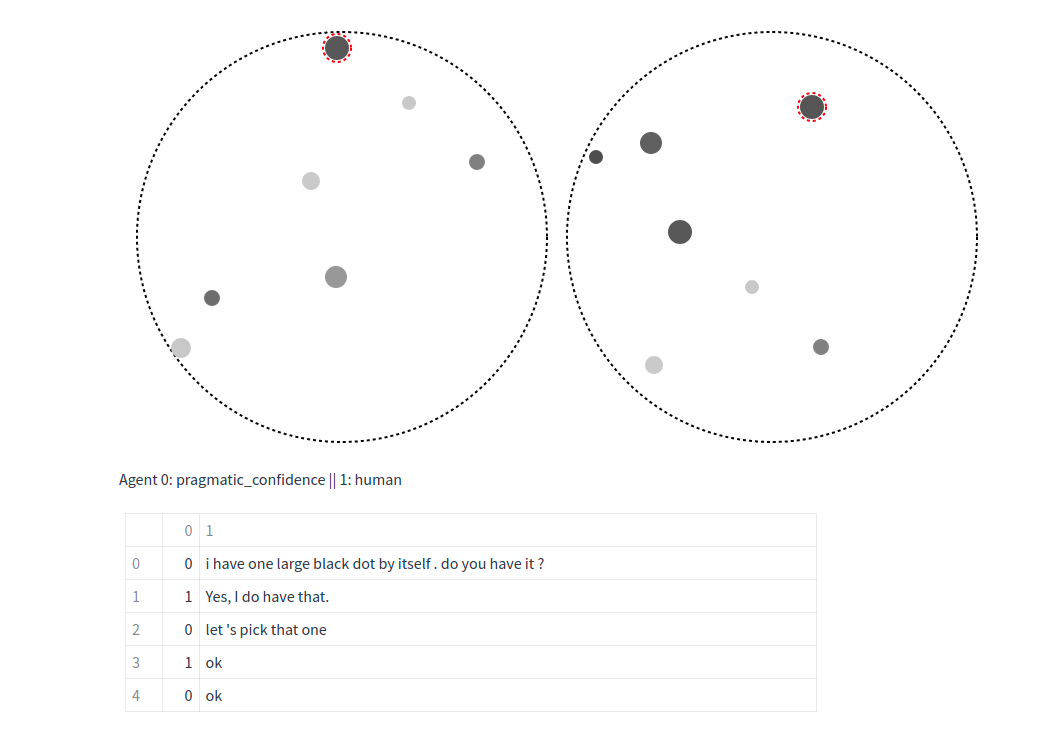
\includegraphics[height=3in]{img/oc-failure.png}
\end{frame}

\begin{frame}
\frametitle{Issue: Scaling rule-based}
\begin{itemize}
\item Rule-based text generation and understanding is somewhat viable for Mutual Friends
    \begin{itemize}
    \item Very optimistic selection, but can be tuned
    \end{itemize}
\item Continuous and spatial nature of OneCommon makes writing rules difficult
    \begin{itemize}
    \item Size, color, and positions all continuous
    \item Descriptions are relative
    \end{itemize}
\end{itemize}
\end{frame}

\begin{frame}
\frametitle{Current approaches: Two extremes}
\begin{itemize}
\item Neural encoder-decoder
    \begin{itemize}
    \item Encode past interactions with a neural net
    \item Generate what to say with a neural net
    \item Brittle strategy, less brittle language
    \end{itemize}
\item Rule-based
    \begin{itemize}
    \item Encode past interactions in a table
    \item Use rules for what to say next
    \item Nonparametric lookup of utterances
    \item Brittle language, less brittle strategy
    \end{itemize}
\item Meet in middle with interpretable planning + neural language
\end{itemize}
\end{frame}


\begin{frame}
\frametitle{A dialogue turn}
\begin{itemize}
\item Engaging in dialogue requires
    \begin{itemize}
    \item Inference: What do I know? How do I represent it?
    \item Planning: What should I do and say?
    \end{itemize}
\item Formulate as model-based optimization
    \begin{itemize}
    \item Plan what to say through a simple model of our partner
    \item Model of partner conditions on past information
    \end{itemize}
\end{itemize}
\end{frame}

\begin{frame}
\frametitle{Problem setup}
\begin{itemize}
\item Goal: Mutually select the same item as partner
    \begin{itemize}
    \item Row in knowledge base, dot
    \item Coordinate through dialogue
    \end{itemize}
\item Given history $h$,
we need to chose an action $a$ by optimizing value
\begin{equation*}
\max_a V(h, a)
\end{equation*}
\item Value $V$ = information gain
    \begin{itemize}
    \item Entropy reduction of item selection probability
    \end{itemize}
\item Represent $h,a$ using attributes
    \begin{itemize}
    \item Columns of knowledge base, spatial configuration of dots
    \end{itemize}
\end{itemize}
\end{frame}


\begin{frame}
\frametitle{Information Gain}
\begin{itemize}
\item A good action should move us closer to game success
\item Game success depends on our knowledge of our partner's context
\item Requires
    \begin{itemize}
    \item Belief distribution over selection item given history $p(i \mid h)$
    \item Partner response model $p(o \mid h, a, i)$
    \end{itemize}
\item Represent a turn as

\begin{center}
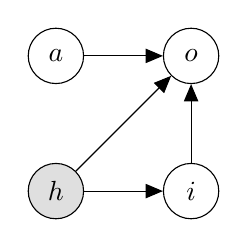
\begin{tikzpicture}
\node[obs] (h) {$h$};
\node[latent, right=of h] (i) {$i$};
\node[latent, above=of i] (o) {$o$};
\node[latent, above=of h] (a) {$a$};
\edge {h} {i};
\edge {h} {o};
\edge {i} {o};
\edge {a} {o};
\end{tikzpicture}
\end{center}
\item Language and planning coupled
\end{itemize}
\end{frame}

\begin{frame}
\frametitle{Decoupling language and planning}
\begin{itemize}
\item Compress actions $a$ and observations $o$ into language and abstract representations
    $\tilde{a}, \tilde{o}$
    \begin{itemize}
    \item Language is high dimensional, redundant, and inefficient for planning
    \end{itemize}
\item Represent a turn as
\begin{center}
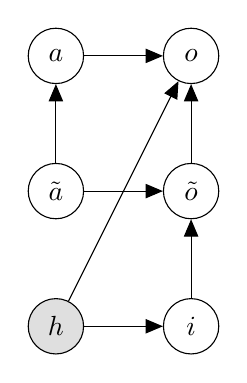
\begin{tikzpicture}
\node[obs] (h) {$h$};
\node[latent, right=of h] (i) {$i$};
\node[latent, above=of i] (to) {$\tilde{o}$};
\node[latent, above=of h] (ta) {$\tilde{a}$};
\node[latent, above=of to] (o) {$o$};
\node[latent, above=of ta] (a) {$a$};
\edge {h} {i};
\edge {h} {o};
\edge {i} {to};
\edge {ta} {a};
\edge {ta} {to};
\edge {to} {o};
\edge {a} {o};
\end{tikzpicture}
\end{center}
\item Abstract observation $\tilde{o} \bigCI h \mid \tilde{a}, i$
\end{itemize}
\end{frame}


\begin{frame}
\frametitle{State and belief: Representation}
\begin{columns}
\begin{column}{0.70\textwidth}
\begin{itemize}
\item History: whether attributes have been confirmed $h \in \set{0,1}^N$
\item Items: $i \in [M], N >> M$
\item Logistic regression with attributes as features
\begin{align*}
p(i \mid h) &= \frac{\exp(\sum_n \psi(h_n, i))}{\sum_{i'} \exp(\sum_n\psi(h_n, i'))}\\
\psi(h_n, i) &= W_{ni} 1(h_n(i))
\end{align*}
\item Learn $W$ on training data
    \begin{itemize}
    \item Many correlated features
    \item Use $\ell_1$ regularization
    \end{itemize}
\item Dialogue = online feature selection
\end{itemize}
\end{column}
\begin{column}{0.30\textwidth}
\centering
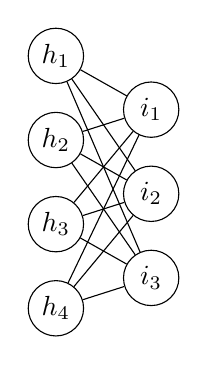
\begin{tikzpicture}
\node[latent] (h1) {$h_1$};
\node[latent, below=1em of h1] (h2) {$h_2$};
\node[latent, below=1em of h2] (h3) {$h_3$};
\node[latent, below=1em of h3] (h4) {$h_4$};
\node[latent, below right=.5em and 2em of h1] (i1) {$i_1$};
\node[latent, below=1em of i1] (i2) {$i_2$};
\node[latent, below=1em of i2] (i3) {$i_3$};

\edge[-] {h1} {i1};
\edge[-] {h1} {i2};
\edge[-] {h1} {i3};
\edge[-] {h2} {i1};
\edge[-] {h2} {i2};
\edge[-] {h2} {i3};
\edge[-] {h3} {i1};
\edge[-] {h3} {i2};
\edge[-] {h3} {i3};
\edge[-] {h4} {i1};
\edge[-] {h4} {i2};
\edge[-] {h4} {i3};
\end{tikzpicture}
\end{column}
\end{columns}
\end{frame}

\begin{frame}
\frametitle{Attributes}
\begin{itemize}
\item Mutual Friends
    \begin{itemize}
    \item Combinations of columns of knowledge base
    \item Name, major, company
    \end{itemize}
\item OneCommon
    \begin{itemize}
    \item Which dots are mentioned
    \item Need to learn lower-level attributes
    \end{itemize}
\item Numerical reasoning?
\end{itemize}
\end{frame}

\begin{frame}
\frametitle{Experiments}
\begin{itemize}
\item Mutual Friends
    \begin{itemize}
    \item Augment rule-based (prior work) to optimize info gain
    \item After OneCommon: Add neural on top
    \end{itemize}
\item OneCommon
    \begin{itemize}
    \item Use attributes = raw mention configurations
        \begin{itemize}
        \item Everything already in system, except for belief / info gain
        \end{itemize}
    \item Learn latent refinement on top of mention configurations
        \begin{itemize}
        \item How to deal with redundancy? (i.e. correlation between features)
        \end{itemize}
    \end{itemize}
\end{itemize}
\end{frame}

\begin{frame}
\frametitle{End}
\end{frame}


\begin{frame}
\frametitle{Concerns}
\begin{itemize}
\item Would a large LM solve all of this?
    \begin{itemize}
    \item Fine tune on small onecommon dataset, are there still repeats?
    \item Unlikely to solve strategy / over optimistism
    \end{itemize}
\end{itemize}
\end{frame}

\begin{frame}
\frametitle{End}
\end{frame}


\begin{frame}
\frametitle{Value: Information Gain}
\begin{itemize}
\item drop slide
\item Picture would be much better here...
\item Value = expected information gain
\begin{align*}
IG(h, a) &= H(i \mid h) - \Es{p(o\mid h,a)}{H(i \mid h, a, o)}\\
\Es{p(o\mid h,a)}{H(i \mid h, a)} &= \sum_o\sum_{i'}p(o\mid h,a,i)p(i\mid h)H(i \mid h,a,o)
\end{align*}
\item Equivalent to minimizing expected uncertainty after receiving a response
\item Cite Yu et al, White et al
\end{itemize}
\end{frame}

\begin{frame}[allowframebreaks]
\frametitle{Citations}
%\printbibliography
\bibliography{anthology.bib,emnlp2020.bib}
\end{frame}

\end{document}
